\documentclass[11pt, a4paper]{jsarticle}
\usepackage{multicol}  % パッケージの追加
\usepackage[dvipdfmx]{graphicx}
\begin{document}
%=============================================================
%=============================================================
\section{Michelson Interferometer and Coherence}
\subsection*{Purpose}
この実験の目的はマイケルソン干渉系によって作られる干渉模様を観測することと,実験で使用しているHe-Neレーザーのコヒーレント長をマイケルソン干渉系を用いて測定することである.
\subsection{Michelson Interferometer}
\subsubsection{Procedure}
まず以下のように干渉系を組み立てる.
\begin{figure}[htbp]
 \begin{center}
  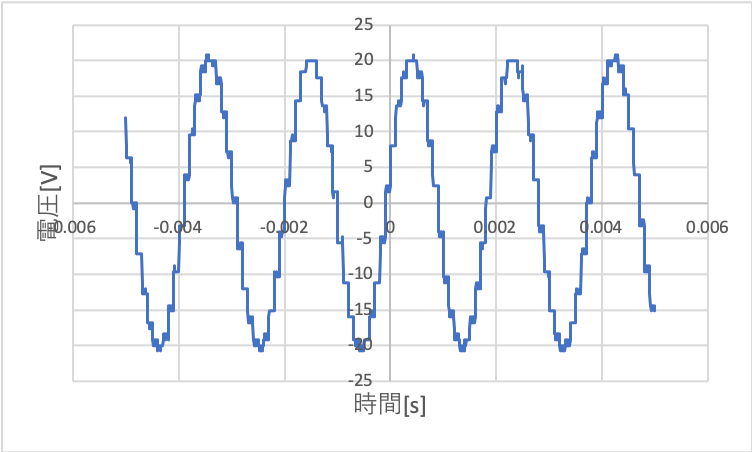
\includegraphics[width=100mm]{fig14.png}
 \end{center}
 \caption{マイケルソン干渉系}
 \label{fig:14}
\end{figure}\\

まず光の強度を弱めるためにNDフィルター(25\%)をレーザーの前に設置する.
次にビームエキスパンダーを組み立てる.
今回はガリレオ型のエキスパンダーを組み立てる.
また,それぞれのミラーの高さを合わせて跳ね返った光がスクリーン上で一致するように調整を行う.
次にM2のミラーを移動させることで干渉縞が観測されたので干渉模様を写真に収める.
さらにその状態から机を叩く事により干渉模様がどのように変化するかを観察する.
その後エキスパンダーの二個目の凸レンズを移動させて二つのレンズ間距離を小さくする事で干渉模様にどのような変化が起きたかを観察する.
得られた干渉縞の写真をカメラに収める.
またこの時$BS-M1 = 8.0cm$,$BS-M2 = 5.0cm$の距離であった.

\subsubsection{Result}
二つの光がスクリーン上で重なり干渉を起こす事で図\ref{fig:15}のような干渉模様が得られた.
また机を叩いて揺れを起こす事でスクリーン上に映っていた干渉模様が消えた.
その後0.98[s]後に元どおりの干渉模様をまた形成した.
さらにエキスパンダーのレンズ間距離を小さくすると干渉模様が図\ref{fig:16}のように円の一部分のように丸くなって映った.
さらにレンズ間距離を元の位置よりも大きくすると同じような円状の干渉模様が得られた.

\begin{figure}[htbp]
 \begin{minipage}{0.45\hsize}
  \begin{center}
   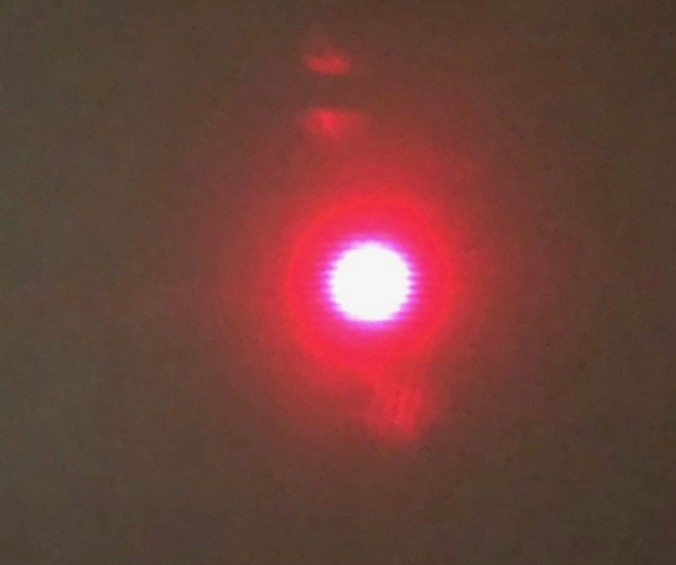
\includegraphics[width=60mm]{fig15.png}
  \end{center}
  \caption{干渉模様}
  \label{fig:15}
 \end{minipage}
 \begin{minipage}{0.45\hsize}
  \begin{center}
   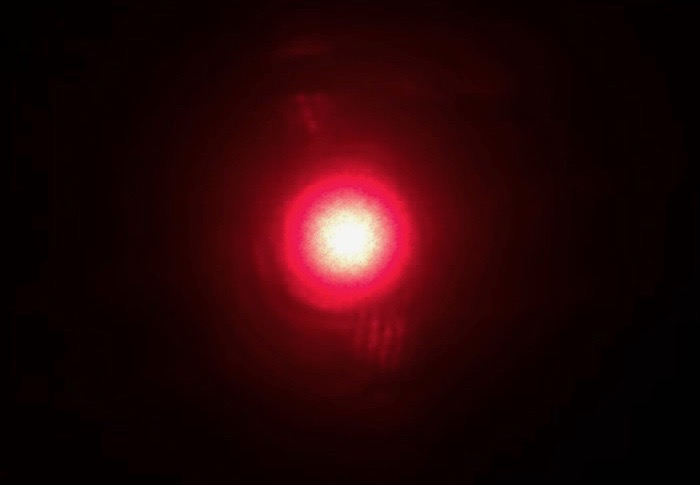
\includegraphics[width=60mm]{fig16.png}
  \end{center}
  \caption{レンズ間を狭くした時の干渉模様}
  \label{fig:16}
 \end{minipage}
\end{figure}

\subsubsection{Discussion}
まずM2の位置を調節する事でスクリーン上に平行な干渉模様が得られたからM1に反射された光とM2に反射された光がそれぞれ平面波であってその波がスクリーン上でぶつかる事によって干渉模様が得られたと考えられる.
この事実から実験で使用したレーザーはコヒーレントな光であると言える.

机を叩いた際に干渉模様が見えなくなったのは叩いた振動によって一時的にそれぞれの光路長が異なりスクリーン上で干渉条件が満たされなくなったためだと考えられる.

またミラーの角度を変えるとスクリーン上で観測される干渉模様の縞の感覚が異なったのは二つのビーム光の入社角度が異なるためだと考えられる.

さらにエキスパンダーのレンズ間距離を縮めた際に同心円状の干渉模様が得られたのは平行光だったビームエキスパンダーによって発散してビーム光が球面波になった為だと考えられる.

またマイケルソン干渉系は二つのビーム光の経路差に強く依存するため光路の途中にガラスなどを挿入することでガラスの屈折率を測定することに応用ができると予測される.

%=============================================================
\subsection{Coherence}
\subsubsection{Procedure}
前回の実験と同様に図\ref{fig:14}の光学系を製作する.初めの$BS-M1 = 8.0cm$,$BS-M2 = 5.0cm$の状態から$BS-M1$の距離のみを次第に広げていきスクリーン状で干渉模様が得られなくなるまで広げていきコヒーレント長を決定する.
\subsubsection{Result}
$BS-M1 = 10.0cm$の時は干渉模様が観測された.しかし$BS-M1 = 12.5cm$にすると干渉模様は見れなくなった.
以上の結果より可干渉光路差は$(|BS-M1|-|BS-M2|) \times 2 = 4.0cm$である事がわかった.
\subsubsection{Discussion}
一般に実験用のビーム光のコヒーレント長は数十cmであるので今回の実験から得られた値とは大きな開きがあった.
この原因としては二つの光の交差する角度が小さかったために干渉模様が得られなかった,調節不足で本当はあったのに観測できなかったなどの理由が考えられる.

%==========================================================
%==========================================================
\newpage
\end{document}
